\section{Point spread function}
\label{sec:PSF}

In the following section, we analyze the point spread function (PSF) by analyzing a 3D stack of 
beats embedded in agarose matrix. This matrix disables movement of the beat. 
As the beats are smaller than the resolution, we can observe diffraction. The diffraction itself 
causes an intensity pattern described by an Airy function as depicted in \cref{fig:Airy}. 

\begin{figure}[h]
    \centering
    \begin{subfigure}{0.51\linewidth}
        \centering
        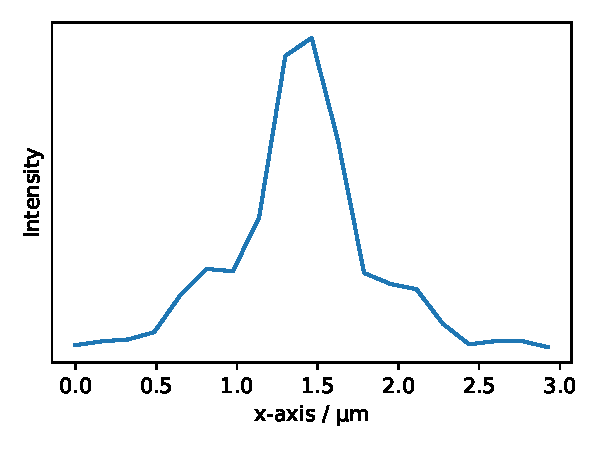
\includegraphics[width = \textwidth]{Bilder/PSF/Airy.pdf}
        \caption{Cut through the picture in \ref*{sub@subfig:AiryBild}}
        \label{subfig:Airy}
    \end{subfigure}
    \hfill
    \begin{subfigure}{0.43\linewidth}
        \centering
        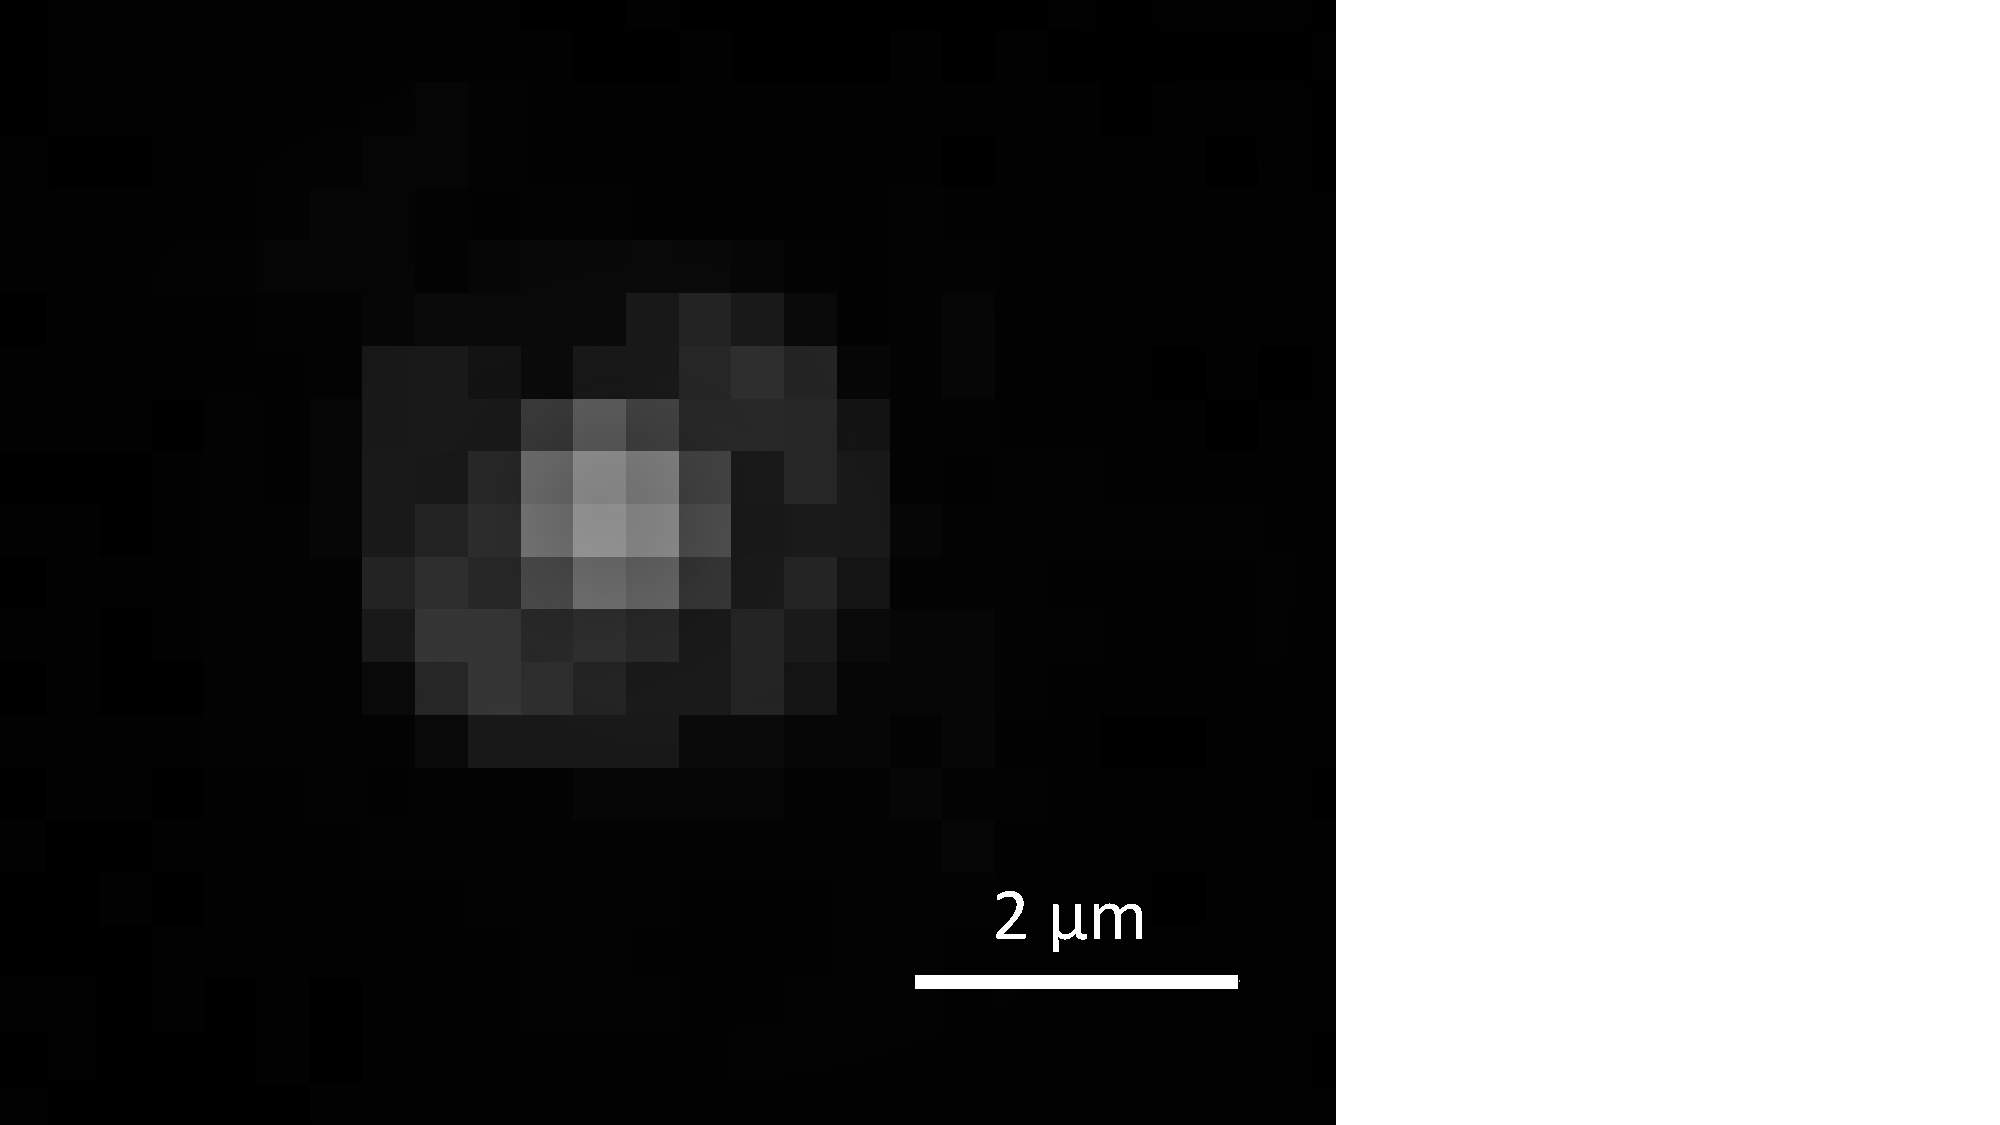
\includegraphics[width = \textwidth]{Bilder/PSF/2DBeugung_cropped.pdf}
        \caption{Image of a beat}
        \label{subfig:AiryBild}
    \end{subfigure}
    \caption{Image of a beat collected with a light sheet microscope (right) and a horizontal cut depicting the intensity profile (left). The intensity profile does have one main peak and two shoulders, which are two separate small peaks.}
    \label{fig:Airy}
\end{figure}